%%%%%%%%%%%%%%%%%%%%%%%%%%%%%%%%%%%%%%%%%%%%%%%%%%%%%%%%%%%%%%%%%%%%%%%%
% Escuela Politécnica Superior de la Universidad de Alicante
% Realizado por: Jose Manuel Requena Plens
% Contacto: info@jmrplens.com / Telegram:@jmrplens
%%%%%%%%%%%%%%%%%%%%%%%%%%%%%%%%%%%%%%%%%%%%%%%%%%%%%%%%%%%%%%%%%%%%%%%%

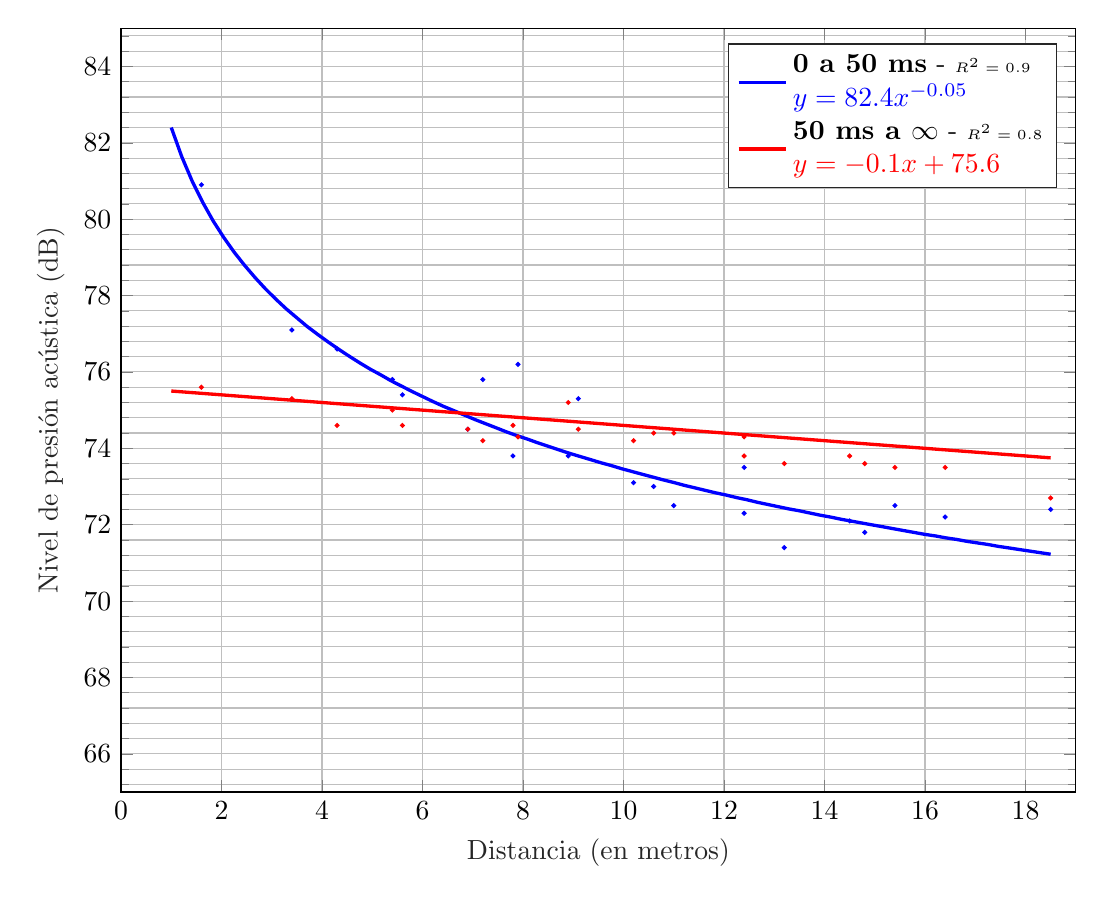
\begin{tikzpicture}

\begin{axis}[%
width=\textwidth,
height=0.8\textwidth,
at={(0\textwidth,0\textwidth)},
scale only axis,
xmin=0,
xmax=19,
xlabel style={font=\color{white!15!black}},
xlabel={Distancia (en metros)},
ymin=65,
ymax=85,
xmajorgrids,
xminorgrids,
ymajorgrids,
yminorgrids,
minor y tick num= 4,
ylabel style={font=\color{white!15!black}},
ylabel={Nivel de presión acústica (dB)},
axis background/.style={fill=white},
%xmajorgrids,
%xminorgrids,
%ymajorgrids,
%yminorgrids,
legend style={legend cell align=left, align=left, draw=white!15!black}
]
\addplot[color=blue,domain=1:18.5, samples=85,line width=1.2]{82.40*x^(-0.05)};
\addlegendentry{\textbf{0 a 50 ms} - \tiny{$R^2 = 0.9$}\\$\color{blue}y = 82.4·x^{-0.05}$}

\addplot[color=red,domain=1:18.5, samples=85,line width=1.2]{-0.1*x+75.6};
\addlegendentry{\textbf{50 ms a $\infty$} - \tiny{$R^2 = 0.8$}\\$\color{red}y = -0.1·x+75.6$}

% Puntos
\addplot [color=blue, only marks,mark size=0.7pt]
  table[row sep=crcr]{%
  1.6	80.9\\
3.4	77.1\\
5.6	75.4\\
7.8	73.8\\
10.2	73.1\\
12.4	72.3\\
14.8	71.8\\
4.3	76.6\\
5.4	75.8\\
6.9	74.5\\
8.9	73.8\\
11.0	72.5\\
13.2	71.4\\
15.4	72.5\\
7.2	75.8\\
7.9	76.2\\
9.1	75.3\\
10.6	73.0\\
12.4	73.5\\
14.5	72.1\\
16.4	72.2\\
18.5	72.4\\
  };
  
  \addplot [color=red, only marks,mark size=0.7pt]
  table[row sep=crcr]{%
  1.6	75.6\\
3.4	75.3\\
5.6	74.6\\
7.8	74.6\\
10.2	74.2\\
12.4	74.3\\
14.8	73.6\\
4.3	74.6\\
5.4	75.0\\
6.9	74.5\\
8.9	75.2\\
11.0	74.4\\
13.2	73.6\\
15.4	73.5\\
7.2	74.2\\
7.9	74.3\\
9.1	74.5\\
10.6	74.4\\
12.4	73.8\\
14.5	73.8\\
16.4	73.5\\
18.5	72.7\\
  };
\end{axis}
\end{tikzpicture}%